\documentclass{article}
\usepackage[utf8]{inputenc}
\usepackage[margin=1in]{geometry}

\usepackage{algorithm}
\usepackage[noend]{algpseudocode}
\usepackage{enumitem}

\usepackage{tikz}
\usetikzlibrary{calc,shapes.multipart,chains,arrows,positioning}
\tikzstyle{vertex}=[draw,fill=myseagreen,circle,minimum size=24pt,inner sep=0pt]
\definecolor{myseagreen}{RGB}{240,240,240}

\title{Strongly Connected Components and Biconnected Components}
\author{Daniel Wisdom}
\date{27 January 2017}

\begin{document}

\maketitle


\begin{figure}[h]
\center
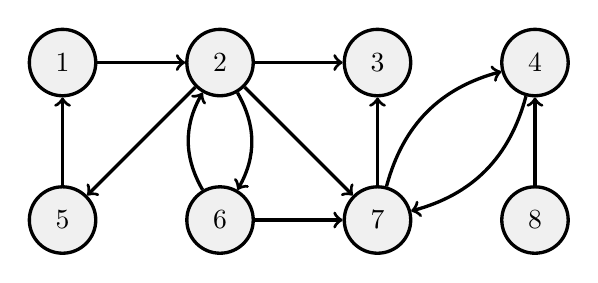
\begin{tikzpicture}[very thick,level/.style={sibling distance=70mm/#1}]
\draw (0, 0) node [vertex] (n1) {5};
\draw (2, 0) node [vertex] (n2) {6};
\draw (4, 0) node [vertex] (n3) {7};
\draw (6, 0) node [vertex] (n4) {8};
\draw (0, 2) node [vertex] (m1) {1};
\draw (2, 2) node [vertex] (m2) {2};
\draw (4, 2) node [vertex] (m3) {3};
\draw (6, 2) node [vertex] (m4) {4};
\draw[->] (m1) -- (m2);
\draw[->] (m2) -- (n1);
\draw[->] (n1) -- (m1);
\draw[->] (n2) edge [bend left] (m2);
\draw[->] (m2) edge [bend left] (n2);
\draw[->] (n2) -- (n3);
\draw[->] (m2) -- (m3);
\draw[->] (m2) -- (n3);
\draw[->] (n3) -- (m3);
\draw[->] (n3) edge [bend left] (m4);
\draw[->] (m4) edge [bend left] (n3);
\draw[->] (n4) -- (m4);
\end{tikzpicture}
\caption{A directed graph. \textit{Credit: Crash Course Coding Companion.}}
\end{figure}

\section{Strongly Connected Components}

A strongly connected component (SCC) is a set of vertices where every vertex can reach every other vertex.  In an undirected graph the SCCs are just the groups of connected vertices.  We can find them using a simple DFS.  This works because, in an undirected graph, $u$ can reach $v$ if and only if $v$ can reach $u$.

This is not true in a directed graph, which makes finding the SCCs harder.  More on that later.

\section{Kernel graph}

We can travel between any two nodes in the same strongly connected component. So what if we replaced each strongly connected component with a single node? This would give us what we call the \textit{kernel graph}, which describes the edges between strongly connected components. Note that the kernel graph is a directed acyclic graph because any cycles would constitute an SCC, so the cycle would be compressed into a kernel.

\begin{figure}[h]
\center
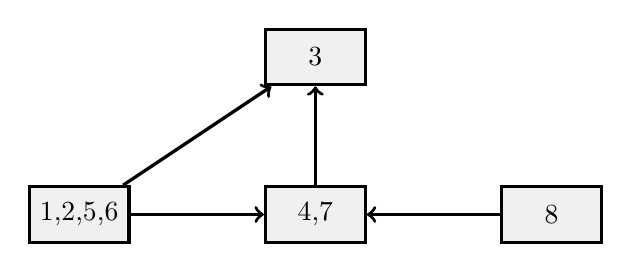
\begin{tikzpicture}[very thick,level/.style={sibling distance=70mm/#1}]
\tikzstyle{vertex}=[draw,fill=myseagreen,rectangle,minimum width=36pt,minimum height=20pt,inner sep=0pt]
\draw (0, 0) node [vertex] (n1) {1,2,5,6};
\draw (3, 0) node [vertex] (n3) {4,7};
\draw (6, 0) node [vertex] (n4) {8};
\draw (3, 2) node [vertex] (n2) {3};
\draw[->] (n1) -- (n3);
\draw[->] (n1) -- (n2);
\draw[->] (n3) -- (n2);
\draw[->] (n4) -- (n3);
\end{tikzpicture}
\caption{Kernel graph of the above directed graph.}
\end{figure}


\section{Tarjan's SCC Algorithm}

In a DFS traversal of the graph every SCC will be a subtree of the DFS tree. This subtree is not necessarily proper, meaning that it may be missing some branches which are their own SCCs.  This means that if we can identify every node that is the root of its SCC in the DFS, we can enumerate all the SCCs.

If a node $v$ can reach another node $u$ which is an ancestor of $v$ in the DFS, then $v$ cannot be the root of an SCC.  This is because there is a cycle between $u$ and $v$.  The DFS from $u$ found $v$, so there is clearly a path from $u$ to $v$.  If the DFS starting at $v$ finds a way to $u$, then $u$ and $v$ must be in the same SCC.  $u$, or some ancestor or $u$, is the root of the SCC.

We can give the nodes an ID by the order we visit them in the DFS.  Every time we visit a new node we will give it the next available ID.  This allows us to define $v$.lowlink as the lowest node ID on the stack that is reachable from $v$.  $v$ can reach itself, so $v$.lowlink is at most $v$.ID. If $v$ can reach anything above it in the stack then $v$ is not the root of its SCC.  If, after recurring on all of $v$ children, $v$.lowlink still equals $v$.ID then $v$ is the root of its SCC.

We will use a stack to keep track of nodes we have already visited.  The stack is different from The Stack which stores all method calls and is responsible for recursion.  The stack in this algorithm is an explicit one we will be keeping.  Whenever we visit a node we will push it onto the stack.  However, we will not always pop a node off when its DFS call returns.  We will only pop nodes off the stack before an SCC root node returns.  This means that when a root node returns, all the nodes in its SCC are above in on the stack.  We can keep popping until we pop off the SCC root node, at which point we output the SCC in whatever format we want.

\begin{algorithm}[H]
\caption{Tarjan's SCC Algorithm}
\begin{algorithmic}
\Function{Visit}{vertex $v$}
    \State $v$.ID = nextID
    \State nextID++
    \State $v$.lowlink = $v$.ID
    \State push $v$ onto the stack
    \State $v$.onStack = true
    \For{Each edge ($v$,$u$)}
        \If{$u$ has not been visited}
            \State Visit($u$)
            \State $v$.lowlink = min($v$.lowlink, $u$.lowlink)
        \ElsIf{$u$.onStack}
            \State $v$.lowlink = min($v$.lowlink, $u$.lowlink)
            \Comment{More on this line later}
        \EndIf
    \EndFor
    
    \If{$v$.lowlink = $v$.ID}
        \While{$v$ is still on the stack}
            \State pop $u$ off the stack
            \State add $u$ to the SCC
            \State $u$.onStack = false
        \EndWhile
    \EndIf
\EndFunction
\end{algorithmic}
\end{algorithm}

Because a DFS staring from one node may not reach every node we must call Visit() on every node that has not yet been visited.  The overall algorithm takes $O(|V| + |E|)$ time.

Note: Tarjan's original algorithm had the noted line as $v$.lowlink = min($v$.lowlink, $u$.ID).  This will also work.  Many online sources use this version to be true to the original.  However, using $u$.lowlink instead of $v$.ID gives us a nice property: $v$ and $u$ are in the same SCC if and only if $v$.lowlink = $u$.lowlink.  Because this can be helpful, I suggest using the $u$.lowlink version.


\section{Biconnected Components}

In an undirected graph biconnected components are sets of nodes where each one is reachable from every other, even if any one node is removed.  Note that one node can be in multiple BCCs, up to its degree.  Take A--B--C:  B is in a biconnected component with A and in one with C.  However, every edge is in exactly one BCC.  We can define BCCs by the edges they include, or by articulation points.  Articulation points are nodes that divide BCCs, and belong to both.  An articulation point is also any node that, when removed, divides the graph into disconnected components.

We will use a similar algorithm with lowlinks to find the articulation points.  In this version we need to use Tarjan's original version of lowlinks, where $v$.lowlink = min($v$.lowlink, $u$.depth) at the line noted.  A node is an articulation point if it has a subtree which cannot reach up the DFS tree past the node.  More formally, a node $v$ is an articulation point if $v$ has a child $u$ with $u$.lowlink $\geq$ $v$.depth.  The only spacial case we have to deal with is the DFS root. If the root has more than one child in the DFS then it is an articulation point.  The root only has multiple subtrees if those subtrees are disconnected, making the root a cut vertex.

When we compress each BCC to a node, with edges for shared articulation points we get the block-cut tree of the graph.  This is an undirected graph, which cannot have cycles because any cycle forms a BCC.

\section{Problems}

\begin{itemize}[leftmargin=0pt]
\item[\label={}]
\textit{Mining Your Own Business} (ICPC World Finals, 2011)

John Digger is the owner of a large illudium phosdex mine. The mine is made up of a series of tunnels
that meet at various large junctions. Unlike some owners, Digger actually cares about the welfare of
his workers and has a concern about the layout of the mine. Specifically, he worries that there may a
junction which, in case of collapse, will cut off workers in one section of the mine from other workers
(illudium phosdex, as you know, is highly unstable). To counter this, he wants to install special escape
shafts from the junctions to the surface. He could install one escape shaft at each junction, but Digger
doesn’t care about his workers that much. Instead, he wants to install the minimum number of escape
shafts so that if any of the junctions collapses, all the workers who survive the junction collapse will
have a path to the surface.
Write a program to calculate the minimum number of escape shafts needed.

\item[\label={}]
\textit{Mowing the Field} (USACO January 2016, Platinum)

In an effort to better manage the grazing patterns of his cows, Farmer
John has installed one-way cow paths all over his farm.  The farm
consists of $N$ fields ($1 \le N \le 100000$), conveniently numbered $1..N$, with each one-way
cow path connecting a pair of fields. For example, if a path connects
from field $X$ to field $Y$, then cows are allowed to travel from $X$ to $Y$
but not from $Y$ to $X$.

Bessie wonders how much grass she will be able to eat if she
breaks the rules and follows up to one path in the wrong direction.
Please compute the maximum number of distinct fields she can visit
along a route starting and ending at field $1$, where she can follow up
to one path along the route in the wrong direction.  Bessie can only
travel backwards at most once in her journey.  In particular, she
cannot even take the same path backwards twice.

\item[\label={}]
\textit{Push A Box} (USACO December 2017, Platinum)

The barn can be modeled as an NxM rectangular grid. Some of the grid cells have hay in them. Bessie occupies one cell in this grid, and a large wooden box occupies another cell. Bessie and the box are not able to fit in the same cell at the same time, and neither can fit into a cell containing hay.

Bessie can move in the 4 orthogonal directions (north, east, south, west) as long as she does not walk into hay. If she attempts to walk to the space with the box, then the box will be pushed one space in that direction, as long as there is an empty cell on the other side. If there is no empty cell, then Bessie will not be able to make that move.

A certain grid cell is designated as the goal. Bessie's goal is to get the box into that location.

Given the layout of the barn, including the starting positions of the box and the cow, and the target position of the box, determine if it possible to win the game.

\end{itemize}

\end{document}
